%%%%%%%%%%%%%%%%%%%% author.tex %%%%%%%%%%%%%%%%%%%%%%%%%%%%%%%%%%%
%
% sample root file for your "contribution" to a contributed volume
%
% Use this file as a template for your own input.
%
%%%%%%%%%%%%%%%% Springer %%%%%%%%%%%%%%%%%%%%%%%%%%%%%%%%%%


% RECOMMENDED %%%%%%%%%%%%%%%%%%%%%%%%%%%%%%%%%%%%%%%%%%%%%%%%%%%
\documentclass[graybox]{svmult}

% choose options for [] as required from the list
% in the Reference Guide

\usepackage{mathptmx}       % selects Times Roman as basic font
\usepackage{helvet}         % selects Helvetica as sans-serif font
\usepackage{courier}        % selects Courier as typewriter font
\usepackage{type1cm}        % activate if the above 3 fonts are
                           % not available on your system
                           
%
\usepackage{makeidx}         % allows index generation
\usepackage{graphicx}        % standard LaTeX graphics tool
                             % when including figure files
\usepackage{multicol}        % used for the two-column index
\usepackage[bottom]{footmisc}% places footnotes at page bottom
\usepackage{amsmath}
\usepackage{listings}
\usepackage{minted}
\usepackage{soul}
\usepackage[utf8]{inputenc}
\usepackage[english]{babel}

% see the list of further useful packages
% in the Reference Guide

\makeindex             % used for the subject index
                       % please use the style svind.ist with
                       % your makeindex program

%%%%%%%%%%%%%%%%%%%%%%%%%%%%%%%%%%%%%%%%%%%%%%%%%%%%%%%%%%%%%%%%%%%%%%%%%%%%%%%%%%%%%%%%%

\begin{document}


\title*{Classical Reinforcement Learning}
\author{by \textbf{jhoang}}


%
% Use the package "url.sty" to avoid
% problems with special characters
% used in your e-mail or web address
%
\maketitle

\abstract{Classical Reinforcement Learning is defined to be the era before 2010. However, readers should understand this definition with a grain of salt. The purpose of this document is to provide a sufficient background of reinforcement learning in order to understand more recent work, which we refer to as modern reinforcement learning. In this document, we will talk about the problem statement of reinforcement learning in comparison to other learning problems, then we will talk about exact methods as well as classical approximation based method to solve reinforcement learning.}


\section{Problem statement}

\subsection{Characteristics of Reinforcement Learning}

In \textbf{supervised learning}, a dataset (often drawn i.i.d from a hidden distribution) is provided by a supervisor. The optimization problem is to maximize a certain loss function, e.g. L2 or cross entropy. While this setup is useful in some problems, it's missing certain characteristics that are crucial to how humans learn things,
\begin{itemize}
 \item There is no supervisor
 \item The feedback from the environment is delayed, not instantaneous 
 \item The experience is sequential, not i.i.d
 \item Agent's actions affect the subsequent data it receives
\end{itemize}

Reinforcement learning tries to address this by stating the problem in a slightly different way. In state of having a stateless, i.i.d dataset, assuming there's an agent with a set of actions $\mathcal{A}$. At each timestep $t$, the agent pick an action $a_t$. Upon receiving the action $a_t$ from the agent, the environment returns an observation $o_{t+1}$ and the reward $r_t$. The objective of the agent is to maximize the cumulative reward $g_t(s_0) = \sum^{\infty} \gamma^t r_t$ starting at some initial state $s_0$

\begin{center}
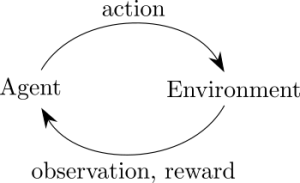
\includegraphics[width=0.5\textwidth]{learning.png}
\end{center}

The strong assumption of reinforcement learning is the \textbf{reward hypothesis}, all goals can be described as maximization of some expected cumulative rewards.  

\subsection{Markov Decision Process (MDP)}
A \textbf{Markov Decision process} is a simpler setup of a reinforcement learning problem. A fully-observable MDP is defined to be a tuple $<S, A, P, r>$, where
\begin{itemize}
\item $S$ is the set of finite states the agent can be in
\item $A$ is the set of finite actions the agent can take at time step $t$
\item $P(s, a, s') = P(s' | s,  a)$ is the probability transition matrix of being in state $s'$ while in state $s$ and taking action $a$
\item $r(s)$ is the reward of ending up in state $s$ 
\item both $P$ and $r$ are visible to the agent
\end{itemize}

Notice that the last condition makes this a fully-observable MDP. Any methods used by the agent with these information is called model-based method, as opposed to model-free methods which don't exploit this information.

\section{Bellman equation and exact solution methods}

It should be immediate to the astute readers that with full knowledge of the environment, we can construct a recursive formula describing the \textbf{dynamics} of the system. First, let's some functions,

\begin{itemize}
\item $\pi$ is the \textbf{policy} of the agent, where $\pi(a | s)$ is the probability distribution over the action space given the current state is $s$
\item $G_t = \sum^{\infty} \gamma^t R_t $, a random variable describing total discounted rewards at time $t$ and initial state $s$. ($R_t$ is the random variable describing reward received at time $t$, note that this is different from $r$ the reward function)
\item $v_{\pi}(s) = E[ G_t | S_t = s ]$ is the state-value function describing the expected total discounted rewards of a state, if the agent follows policy $\pi$
\item $q_{\pi}(s, a) = E[G_t| S_t = s, A_t = a ]$, the action-value function describing the expected total discounted rewards of a state-action pair, if the agent follows policy $\pi$
\end{itemize}

A recursive formula, a.k.a Bellman equation, can be immediately derived,

\[
v_{\pi}(S_t) = E[G_t | S_t ] = E[\sum^{\infty} \gamma^t R_t | S_t  ] 
                      = E[R_t + \gamma G_{t+1}) | S_t ] 
                      = E[R_t + \gamma v_{\pi}(S_{t+1}) | S_t ]
\]

Similarly, for action-value function,

\[
q_{\pi}(S_t, A_t) = E[G_t | S_t, A_t] = E[\sum^{\infty} \gamma^t R_t | S_t, A_t] 
                      = E[R_t + \gamma G_{t+1} | S_t, A_t] 
                      = E[R_t + \gamma Q_{\pi}(S_{t+1}, A_{t+1}) | S_t, A_t]
\]

The Bellman expectation equation tells us the relationship between the action-value function and the state-value function,

$v_{\pi}(s) = E_{\pi}[q_{\pi}(s, a) ] = \sum_{a \in A}  \pi (a | s) q_{\pi}(s, a) $, and $q_{\pi}(s, a) = R^{a}_{s} + \gamma \sum_{s' \in S} P(s, a, s') v_{\pi}(s')$. 

So, $v_{\pi}(s) = E_{\pi}[q_{\pi}(s, a) ] = \sum_{a \in A}  \pi (a | s) q_{\pi}(s, a) =  \sum_{a \in A}  \pi (a | s) (R^{a}_{s} + \gamma \sum_{s' \in S} P(s, a, s') v_{\pi}(s'))$

This tells us that if we fix the policy $\pi$ we can use dynamic programming to work backward from the terminal state and find the value function (and action-value function) for all states and actions. The natural idea is to start with a random policy, then evaluate the value function with the equation above, then improve the new policy by acting greedily with respect to the value function, and repeat until convergence. This is called policy iteration. The idea can be demonstrated in the picture and the code below,

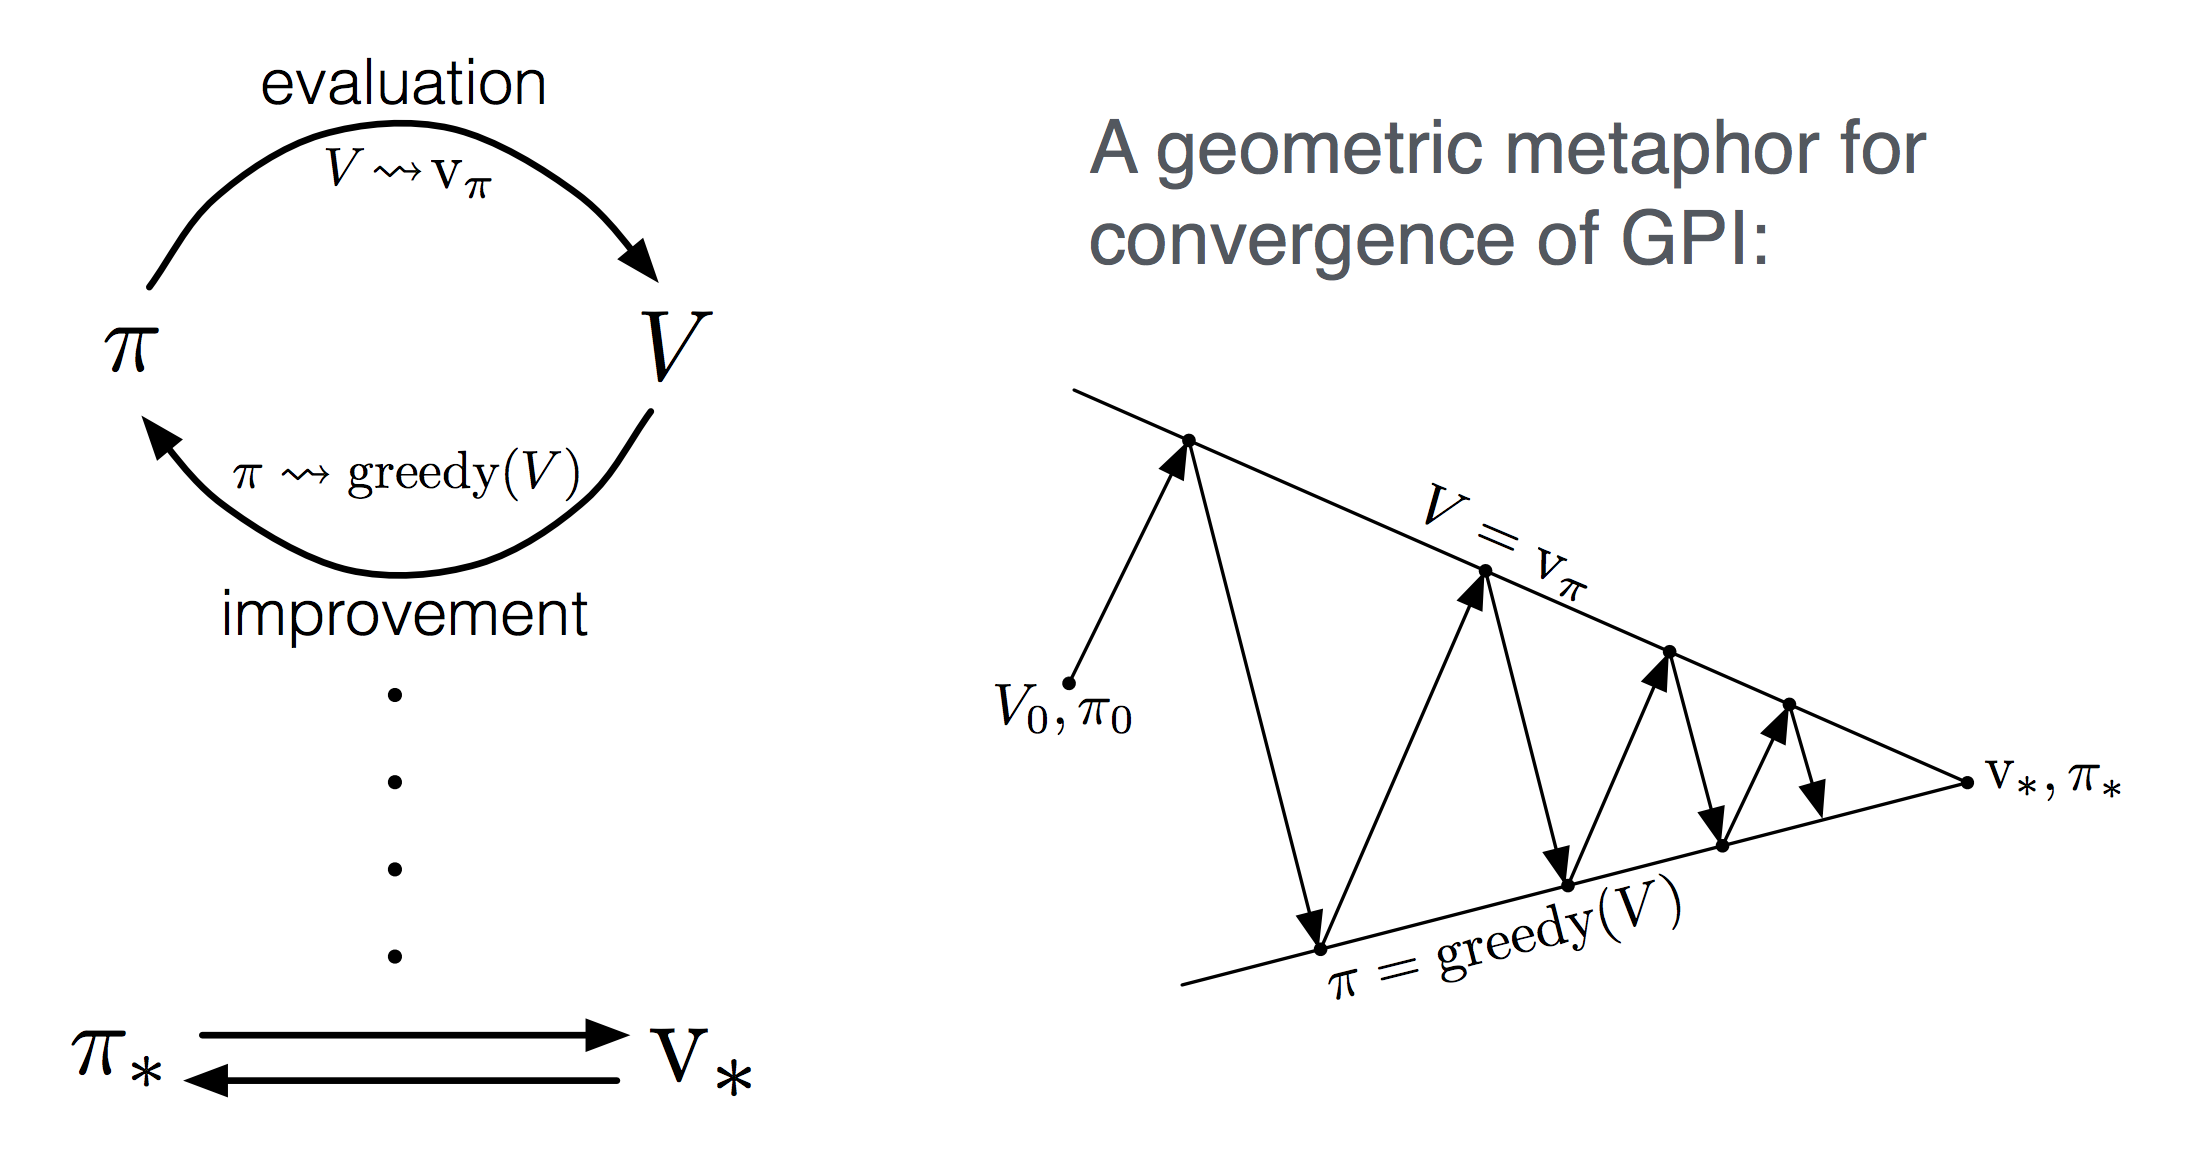
\includegraphics[width=\textwidth]{policy_iter.png}


\begin{minted}[mathescape, linenos, numbersep=5pt, gobble=2, frame=lines, framesep=2mm]{python}
  def policy_eval(policy, env, discount_factor=1.0, theta=0.00001):
    """
    Evaluate a policy given an environment and a full description 
    of the environment's dynamics.

    Args:
        policy: [S, A] shaped matrix representing the policy.
        env: OpenAI env. env.P represents the transition 
        probabilities of the environment.
            env.P[s][a] is a list of transition tuples (
            prob, next_state, reward, done).
            env.nS is a number of states in the environment.
            env.nA is a number of actions in the environment.
        theta: We stop evaluation once our value function 
        change is less than theta for all states.
        discount_factor: Gamma discount factor.

    Returns:
        Vector of length env.nS representing the value function.
    """
    # Start with a random (all 0) value function
    V = np.zeros(env.nS)
    while True:
        delta = 0
        # For each state, perform a "full backup"
        for s in range(env.nS):
            v = 0
            # Look at the possible next actions
            for a, action_prob in enumerate(policy[s]):
                # For each action, look at the possible next states...
                for  prob, next_state, reward, done in env.P[s][a]:
                    # Calculate the expected value
                    v += action_prob * prob * (reward + \ 
                            discount_factor * V[next_state])
            # How much our value function changed 
            # (across any states)
            delta = max(delta, np.abs(v - V[s]))
            V[s] = v
        # Stop evaluating once our value function change is 
        # below a threshold
        if delta < theta:
            break
    return np.array(V)
\end{minted}

\begin{minted}[mathescape, linenos, numbersep=5pt, gobble=2, frame=lines, framesep=2mm]{python}
  def policy_improvement(env, policy_eval_fn=policy_eval, discount_factor=1.0):
    """
    Policy Improvement Algorithm. Iteratively evaluates 
    and improves a policy until an optimal policy is found.

    Args:
        env: The OpenAI envrionment.
        policy_eval_fn: Policy Evaluation function that takes 
        3 arguments:
            policy, env, discount_factor.
        discount_factor: gamma discount factor.

    Returns:
        A tuple (policy, V).
        policy is the optimal policy, a matrix of shape [S, A] 
        where each state s contains a valid probability 
        distribution over actions. V is the value function 
        for the optimal policy.

    """
    # Start with a random policy
    policy = np.ones([env.nS, env.nA]) / env.nA

    while True:
        # Evaluate the current policy
        V = policy_eval_fn(policy, env, discount_factor)

        # Will be set to false if we make any changes to the policy
        policy_stable = True

        # For each state...
        for s in range(env.nS):
            # The best action we would take under the currect policy
            chosen_a = np.argmax(policy[s])

            # Find the best action by one-step lookahead
            # Ties are resolved arbitarily
            action_values = np.zeros(env.nA)
            for a in range(env.nA):
                for prob, next_state, reward, done in env.P[s][a]:
                    action_values[a] += prob * (reward + \
                          discount_factor * V[next_state])
            best_a = np.argmax(action_values)

            # Greedily update the policy
            if chosen_a != best_a:
                policy_stable = False
            policy[s] = np.eye(env.nA)[best_a]

        # If the policy is stable we've found an optimal policy. 
        # Return it
        if policy_stable:
            return policy, V
\end{minted}

\begin{theorem}
Policy iteration converges to an optimal policy.
\end{theorem}

\begin{proof}
TODO(jhoang): proof
\end{proof}

Similarly, if we know the optimal value function for all the subproblems $v_{*}(s')$, then we can find $v_{*}(s)$ by doing one-step look ahead, $v_{*}(s) = max_{a \in A} (R^{a}_s + \gamma \sum_{s' \in S} P^a_{ss'} v_{*}(s')$. Therefore, we can iterate directly on the value function,

\begin{minted}[mathescape, linenos, numbersep=5pt, gobble=2, frame=lines, framesep=2mm]{python}
 def value_iteration(env, theta=0.0001, discount_factor=1.0):
    """
    Value Iteration Algorithm.

    Args:
        env: OpenAI env. env.P represents the transition probabilities 
        of the environment.
            env.P[s][a] is a list of transition tuples 
                 (prob, next_state, reward, done).
            env.nS is a number of states in the environment.
            env.nA is a number of actions in the environment.
        theta: We stop evaluation once our value function change 
            is less than theta for all states.
        discount_factor: Gamma discount factor.

    Returns:
        A tuple (policy, V) of the optimal policy and the optimal 
        value function.
    """

    def one_step_lookahead(state, V):
        """
        Helper function to calculate the value for all action in a 
        given state.

        Args:
            state: The state to consider (int)
            V: The value to use as an estimator, Vector of length env.nS

        Returns:
            A vector of length env.nA containing the expected value 
            of each action.
        """
        A = np.zeros(env.nA)
        for a in range(env.nA):
            for prob, next_state, reward, done in env.P[state][a]:
                A[a] += prob * (reward + discount_factor * V[next_state])
        return A

    V = np.zeros(env.nS)
    while True:
        # Stopping condition
        delta = 0
        # Update each state...
        for s in range(env.nS):
            # Do a one-step lookahead to find the best action
            A = one_step_lookahead(s, V)
            best_action_value = np.max(A)
            # Calculate delta across all states seen so far
            delta = max(delta, np.abs(best_action_value - V[s]))
            # Update the value function
            V[s] = best_action_value
        # Check if we can stop
        if delta < theta:
            break

    # Create a deterministic policy using the optimal value function
    policy = np.zeros([env.nS, env.nA])
    for s in range(env.nS):
        # One step lookahead to find the best action for this state
        A = one_step_lookahead(s, V)
        best_action = np.argmax(A)
        # Always take the best action
        policy[s, best_action] = 1.0

    return policy, V
\end{minted}


\section{Monte Carlo methods}

\subsection{MC}

In previous sections, we've seen exact-solution methods (value iteration, policy iteration) in solving fully-observable MDP. However, in real-world, most interesting problems aren't fully-observable, i.e. the agent doesn't have access to the state transition matrix and reward of the environment. In this section, we'll explore model-free method,

First, let's restate the MDP setup without the full-observable condition. A partially-observable MDP is defined to be a tuple $<S, A, P, r>$, where
\begin{itemize}
\item $S$ is the set of finite states the agent can be in
\item $A$ is the set of finite actions the agent can take at time step $t$
\item $P(s, a, s') = P(s' | s,  a)$ is the probability transition matrix of being in state $s'$ while in state $s$ and taking action $a$
\item $r(s)$ is the reward of ending up in state $s$ 
\item \st{both $P$ and $r$ are visible to the agent}
\end{itemize}

Even though, we can't really reuse the exact equation, we may reuse the idea of policy iteration and value iteration. Note that greedy policy improvement is model-free. We only have to find a way to do policy evaluation model-free. Recall the definition of the state-value function,  $v_{\pi}(s) = E_{\pi}[G_t | S_t = s]$. The idea of Monte Carlo method is to use empirical mean to estimate the true expectation, and by law of large number, this empirical mean will converge to the true value. Concretely, there are two Monte Carlo methods, \textbf{first-visit} Monte Carlo and \textbf{every visit} Monte Carlo,

In first-visit Monte Carlo, for multiple episodes, at the end of each episode,
\begin{itemize}
\item To evaluate state $s$
\item First time $t$ that state $s$ is visited in an episode
\item Increment $N(s)$
\item Increment total return $S(s) += G_t$
\item Set $V(s) = S(s) / N(s)$
\end{itemize}

In every-visit Monte Carlo, for multiple episodes, at the end of each episode,
\begin{itemize}
\item To evaluate state $s$
\item Every time $t$ that state $s$ is visited in an episode
\item Increment $N(s)$
\item Increment total return $S(s) += G_t$
\item Set $V(s) = S(s) / N(s)$
\end{itemize}

MC can only work with problems that are episodic, i.e. there must exist a terminal state. MC waits until the end of an episode to update the value function.

TODO(jhoang): code for blackjack example

\subsection{Temporal Difference (TD) learning}

Another way to view Monte Carlo algorithm is to think in terms of incremental update. The MC algorithm is equivalent to, $V(s) = V(s) + \frac{1}{N(s)} (G_t - V(s))$, i.e. incrementally updating the value function towards the target $G_t$. However, as mentioned in previous section, this $G_t$ requires the existence of a terminal state, and delaying the update of the value function to the end of the terminal state. Instead, we can substitute this with a first order estimate, $R_{t+1} + \gamma V(S_{t+1})$,

The TD(0) algorithm,
\begin{itemize}
\item To evaluate state $s$
\item Every time $t$ that state $s$ is visited in an episode
\item Update $V(S_t) = V(S_t) + \alpha (R_{t+1} + \gamma V(S_{t+1} - V(S_t))$ 
\end{itemize}

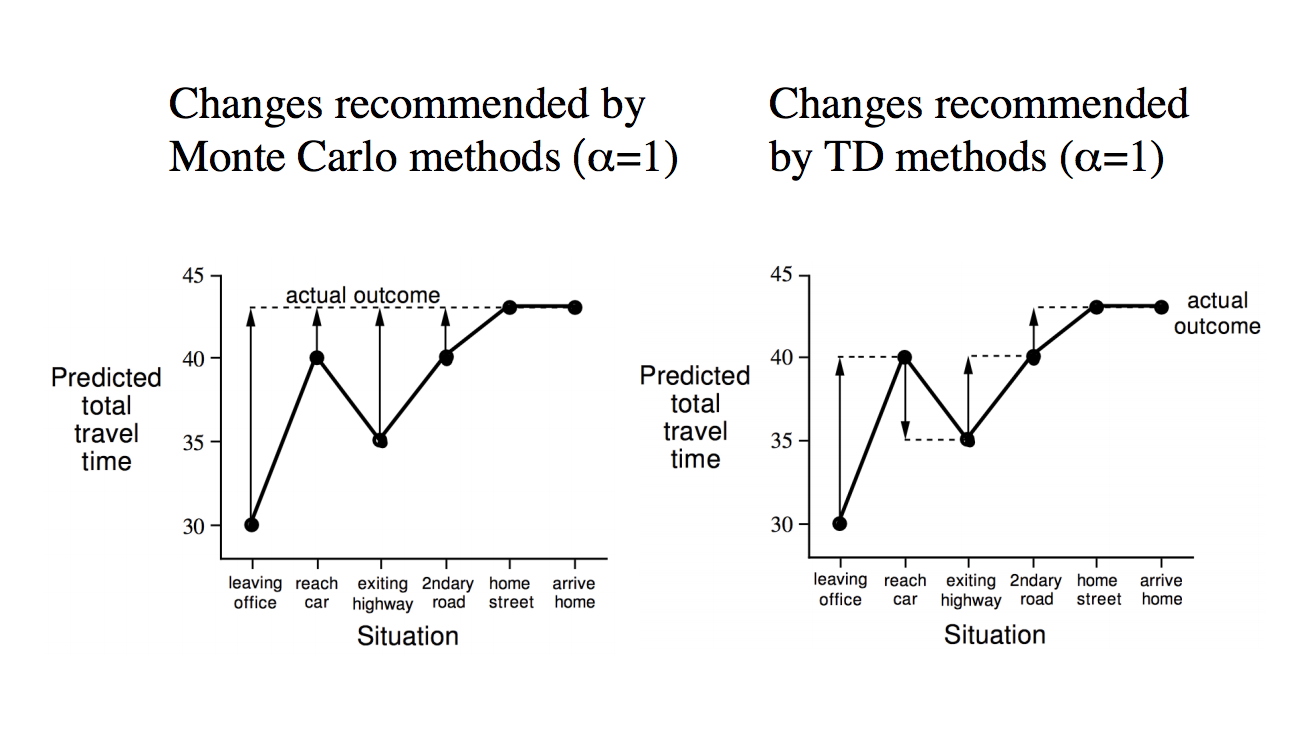
\includegraphics[width=\textwidth]{mctd.png}

TD learns online so it can learn without knowing the final outcome. We can observe that MC is unbiased because $v_{\pi}(S_t) = E[G_t | S_t]$ then $G_t$ is an unbiased estimator of the true value function. Because $v_{\pi}(S_t) = E[R_{t+1} + \gamma v_{\pi}(S_{t+1})| S_t]$ so $R_{t+1} + \gamma v_{\pi}(S_{t+1})$ is an unbiased estimator of the true value function. However, if we replace the true value function $v_{\pi}(S_{t+1})$ with an estimate $V(S_{t+1})$ then the estimator is biased, so TD(0) is biased. We can say the tradeoff between MC and TD(0) is a bias/variance tradeoff, MC is unbiased but high variance, TD(0) is low variance but some biased.


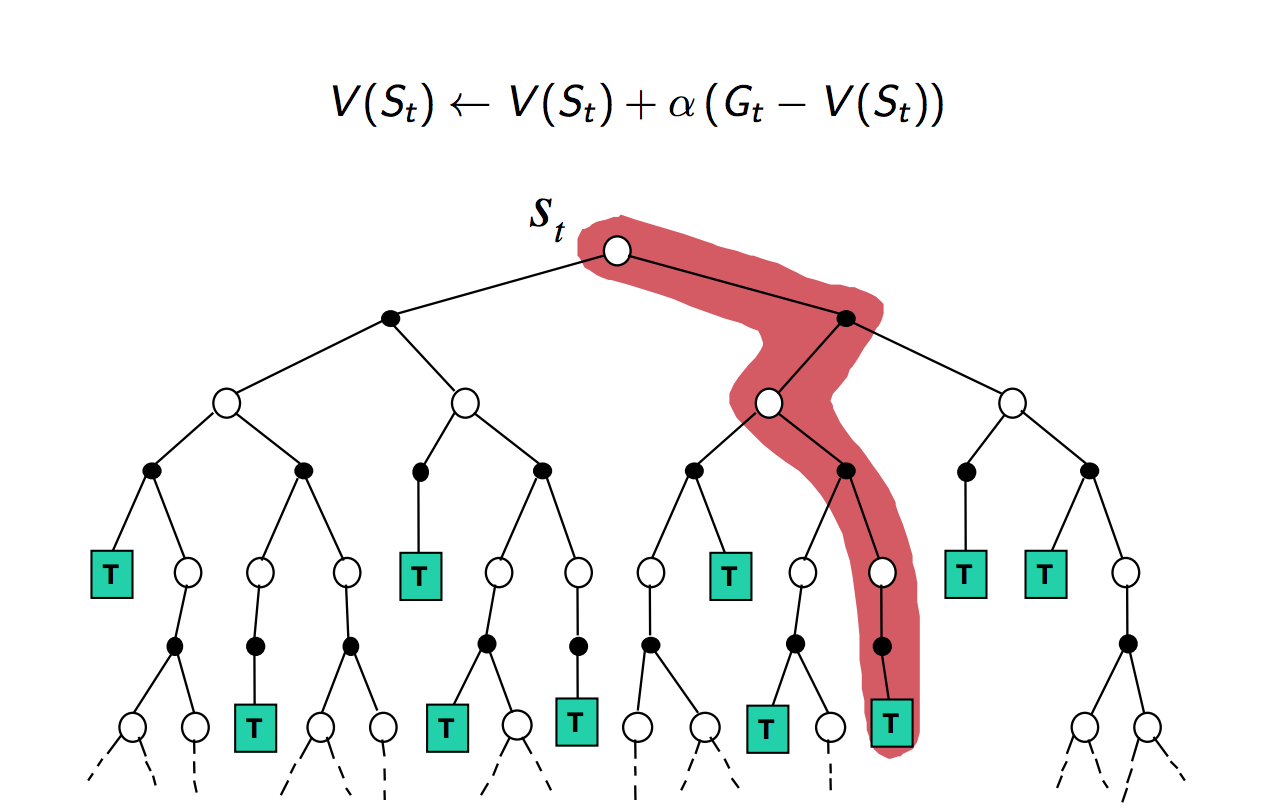
\includegraphics[width=\textwidth]{mc.png}

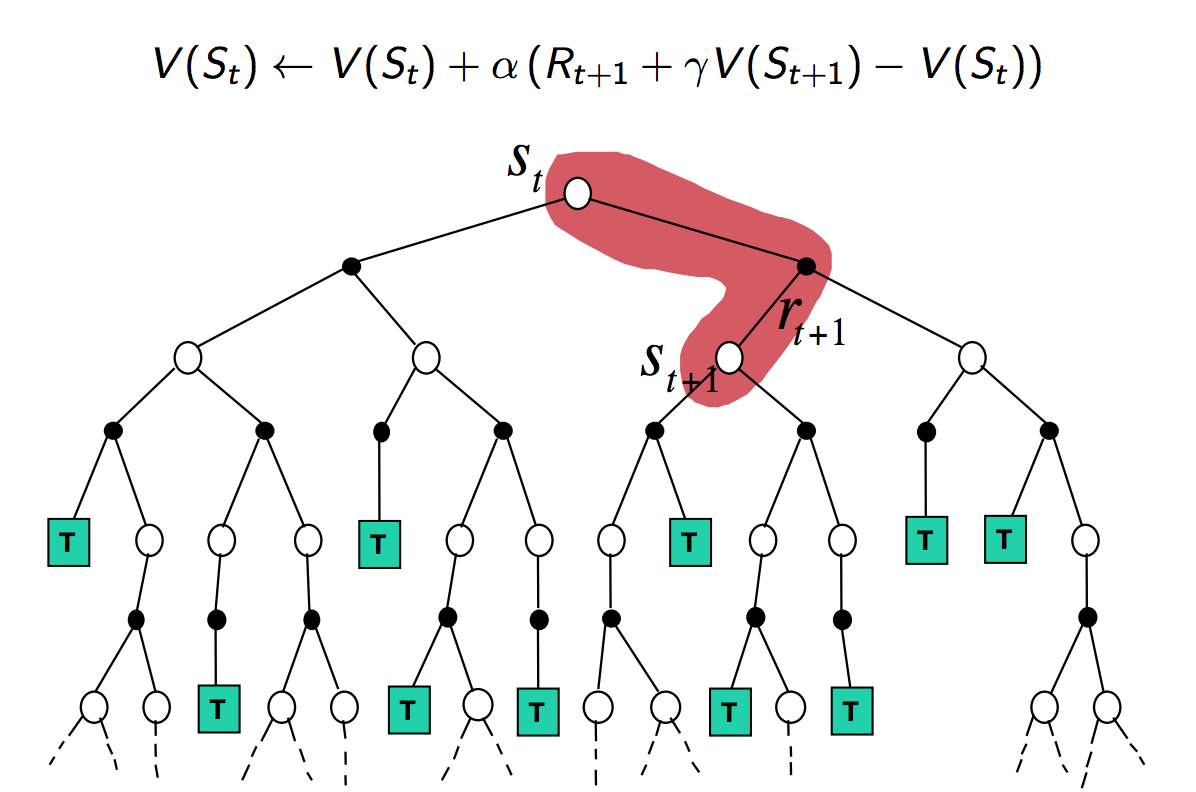
\includegraphics[width=\textwidth]{td.png}

\subsection{TD($\lambda$)}

The idea of forward view $TD(\lambda)$ is to combine all n steps look ahead $G^{(n)}_t = R_{t+1} + \gamma R_{t+2} + .. + \gamma^nV(S_{t+n})$ into one single update target, $G^{\lambda}_t = (1-\lambda)\sum^{\infty}_{n}\lambda^n G^{(n)}_t$. Adjusting $\lambda$ is making an intentional tradeoff between bias and variance.

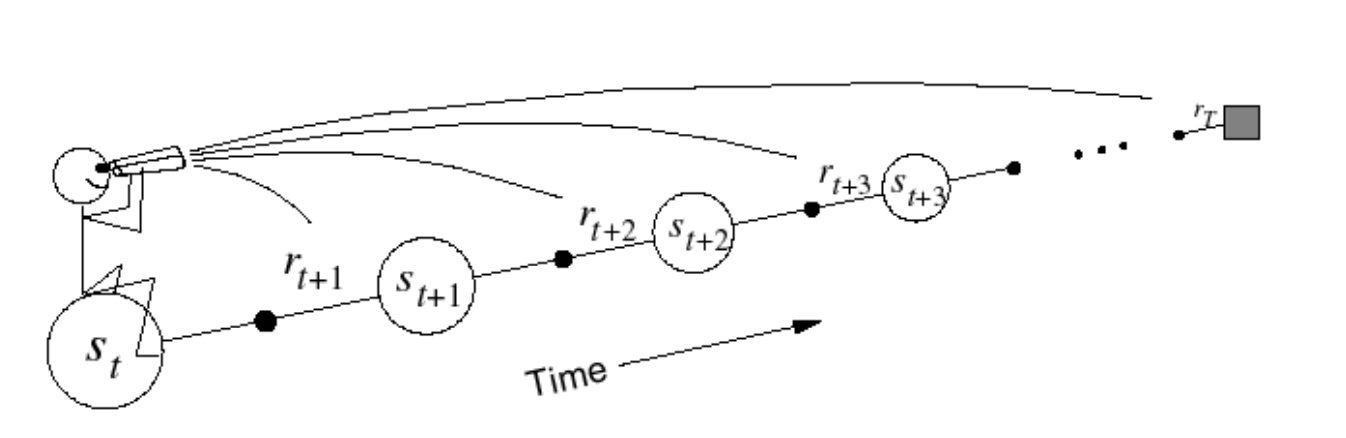
\includegraphics[width=\textwidth]{forward.png}

\section{Policy Gradient methods}

So far, most of the methods we've seen try to find the policy indirectly via a value function (or action-value function). Howeve,r these methods suffer from several drawbacks, 

\begin{itemize}
\item 
\end{itemize}

Policy gradient method tries to learn the policy directly from an episode of experience. Concretely, suppose $\tau = s_0, a_0, s_1, a_1, .. , s_N, a_N$ a rollout of a policy $\pi_{\theta}$. We wish to find $\theta$ maximizing the reward of the rollout,

\begin{center}
 $U(\theta) = E[R(\tau) | \theta] = E[\sum \gamma^t R(s_t, a_t) | \theta]$
\end{center}

Notice that,

\begin{equation}
\begin{split}
\nabla_{\theta} U(\theta) & = \nabla_{\theta} E[\sum \gamma^t R(s_t, a_t) | \theta]  \\
 & = \nabla_{\theta} \sum_{\tau'} P(\tau' | \theta) \sum \gamma^t R^s_t, a_t) \\ & = \sum_{\tau'} P(\tau' | \theta) \nabla_{\theta} \log P(\tau' | \theta) \sum \gamma^t R(s_t, a_t) \\ & = E[ \nabla_{\theta} \log P(\tau' | \theta) \sum \gamma^t R(s_t, a_t) | \theta]  \\ & = E[ \nabla_{\theta} \log (\prod_i P(s_{i+1} | s_i, a_i) \prod_i \pi_{\theta} (a_i | s_i)) \sum \gamma^t R(s_t, a_t) | \theta] \\ & = E[ \nabla_{\theta} \log \prod_i \pi_{\theta} (a_i | s_i)) \sum \gamma^t R(s_t, a_t) | \theta] \\ & = E[ \sum_i \nabla_{\theta}  \log \pi_{\theta} (a_i | s_i)) \sum \gamma^t R(s_t, a_t) | \theta]
\end{split}
\end{equation}

This is called the likelihood ratio gradient. There are two spectacular things about this equation,

\begin{itemize}
\item The gradient of the reward function doesn't depend on the dynamics of the environment. This method is model-free
\item The reward function does not have to be continuous and can also be stochastic, because we only have to take gradient of our policy
\end{itemize}

The problem with updating policy using one rollout is high variance. Actor-critic method and similar methods are variants of policy gradient method aim to solve this problem. There are two main ideas,

\begin{itemize}
\item We can introduce an unbiased quantity (we call a baseline) that helps reduce the variant. Concretely, if $\nabla_{\theta}E_{\tau}[b | \theta] = 0$. Then we can estimate the gradient using $E[ \sum_i \nabla_{\theta}  \log \pi_{\theta} (a_i | s_i)) (\sum \gamma^t R(s_t, a_t) - b) $, which has lower variance. One popular choice of baseline is the state-value function $V^{\pi}$, so the objective function becomes $U(\theta) = E[R(\tau) | \theta] = E[\sum \gamma^t R(s_t, a_t) - V^{\pi}(s_0)| \theta]$
\item We may want to average across multiple rollouts then take the gradient. If we fix the first state and action, then the quantity in interest becomes the state-action value. If we define the advantage function $A^{\pi}_t = Q^{\pi}(s_t, a_t) - V^{\pi}(s_t)$. Then another candidate for loss function can be,  $U(\theta) = E[R(\tau) | \theta] = E[A^{\pi}_t | \theta]$. We will go into more details about these methods in subsequent paper notes.
\end{itemize}
\end{document}

